\begin{frame}{Activité: le plus court chemin}
  


  \begin{block}{Matériel nécessaire}
    \begin{itemize}
    \item Une planche avec des trous au hasard
    \item Autant de longs clous que de trous
    \item Une ficelle suffisamment longue
    \item Un marqueur
    \end{itemize}
  \end{block}

  \begin{block}{Règles du jeu}
    \begin{itemize}
    \item \structure{Situation initiale:} les clous sont mis dans les trous et leurs têtes dépassent de la planche
    \item \structure{Coups autorisés:}
      \begin{itemize}\normalsize
      \item On part d'un clou au hasard et on passe la ficelle de clou en clou
      \item On doit passer par tous les clous
      \item On ne peut passer qu'une seule fois par le même clou
      %\item On peut passer plusieurs fois par le même clou
      \item On doit revenir au point de départ
      \end{itemize}
    \item  \structure{Situation finale:} L'objectif est de passer par tous les
    clous en faisant le plus court chemin. À chaque fois qu'un record est
    battu, on fait une marque sur la ficelle.
    \end{itemize}
  \end{block}

  \bigskip
  \begin{block}{Objectif de l'activité}
    \begin{itemize}
    \item Certains algorithmes sont trop compliqués pour trouver la
    \alert{solution optimale} en un temps \alert{raisonnable}. Parfois, il
    vaut mieux trouver une solution approchée très rapidement, c'est une \alert{heuristique}
    \item algos NP, NP-difficiles, NP-complets
    \item C'est un problème qui parait bête mais qui est complexe et qui a de nombreuses applications dans la vie réelle
    \item Exemple d'application amusante de notion de NP-complétude:  \url{http://arxiv.org/abs/1203.1895}
    \end{itemize}
  \end{block}

\end{frame}

\begin{frame}{Ce qu'il faut retenir du plus court chemin}
  \centerline{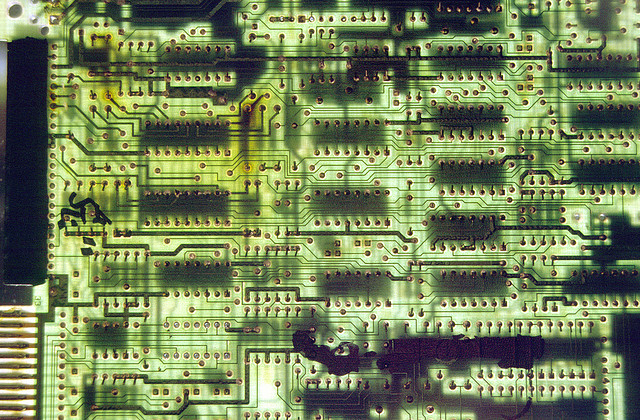
\includegraphics[width=.7\linewidth]{img/electric_city.jpg}\label{img:electric:city}}
  
\end{frame}
